\section{Application to the COVID-19 outbreak}

The model described in Section~\ref{sec:model} is tuned here to fit at best the dataset from Lombardy shown in Figure~\ref{fig:data_lombardy}. Since the data available show just the leading curve of the outbreak, only parameters $\beta$, $\braket{k}$, $\delta$ and $\tau$ have to be tuned. Moreover, an additional parameter $t_0$ has been added to shift the distribution in time. The available dataset regards the \emph{total cases}, corresponding to the sum of infected (positively tested), recovered and deaths. This is not immediately comparable with the population classes in the model. Here it is identified as the sum of quarantined, recovered and deaths. Infected population is not included in the total number because it would correspond to the whole infected population being tested as positive, even the population not showing symptoms, highly probable in young population. Therefore the infected population correspond to the part of the population that has the virus but has not been tested, and all the positively tested population is immediately quarantined. The best fitting setup is shown in Figure~\ref{fig:data_vs_model_first_lombardy}. Parameters modifying the trailing edge of the infection is set to approximate values of the outbreak. Mortality is set to $2\%$, reinfection probability to $10^{-5}$ since yet no cases have been observed. Population is set to $10^7$, corresponding to Lombardy population.

\begin{figure}
\centering
  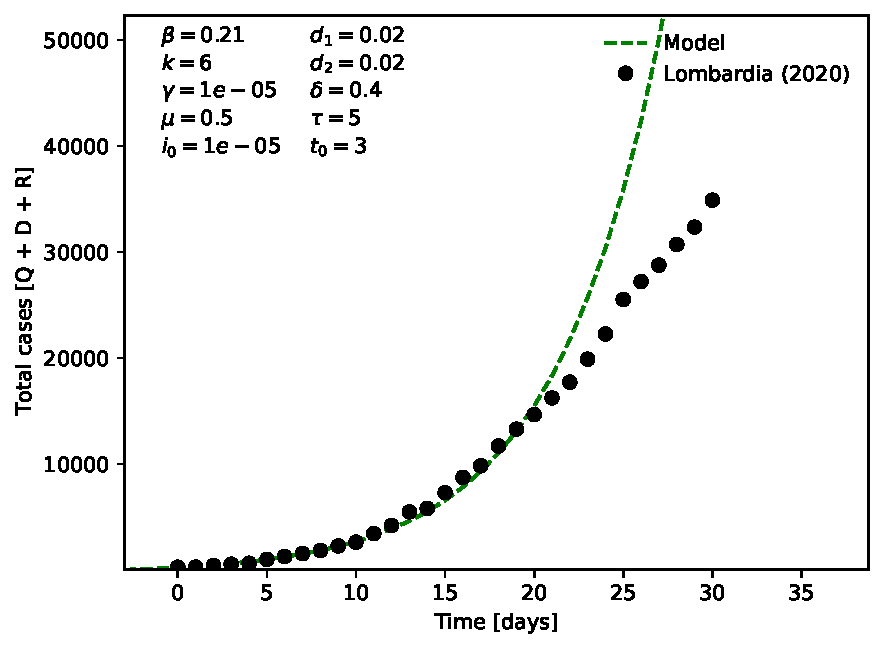
\includegraphics[width=0.4\textwidth]{imgs/Covid/DataVsModel_parameters_Lombardia_less_impacting.pdf}
  \caption{Best match of parameters to make the model described in Section~\ref{sec:model} fit with data il Lombardy.}
  \label{fig:data_vs_model_first_lombardy}
\end{figure}
